% Written by Kamila Larripa, August 2020 for Math 102
\documentclass[12pt]{amsart}
\usepackage{amssymb, latexsym,xspace}
\usepackage[pdftex]{graphicx}
\usepackage{amsmath}
\usepackage{soul} % for highlights-- command is \hl
\usepackage{xcolor}

%%%%%%%%%%%%%%%%%%%%%%%
%
% Change course, date, etc. here and the 
% header will be automatically generated.
%
%%%%%%%%%%%%%%%%%%%%%%%
\newcommand{\class}{Math 102}
\newcommand{\term}{Precalculus}
\newcommand{\quiztitle}{Problem Set 3: Transformations of the Graph of a Function}
%%%%%%%%%%%%%%%%%%%%

% long division symbol
\newcommand\Mydiv[2]{%
$\strut#1$\kern.25em\smash{\raise.3ex\hbox{$\big)$}}$\mkern-8mu
        \overline{\enspace\strut#2}$}
        
        %use like this  \Mydiv{56}{3678}\quad\Mydiv{3}{37678}


%%%%%% Small margin to leave room for students' work %%%%%%%
\usepackage[margin=0.75in,top=0.5in,
            nohead,
            pdftex]{geometry}

%%%%%% Various PDF commands; generally not needed in a quiz %%%%%%%
\usepackage[pdftex, colorlinks=true,
            linkcolor=blue, citecolor=blue,
            urlcolor=blue, letterpaper,
            pdftitle={},
            pdfpagemode=None]{hyperref}

%%%%% spread the lines out a bit.
\pagestyle{plain}
\linespread{1.3}
\parindent 0ex

\begin{document}
%%%%%%%%% Header %%%%%%%%%%%
\textbf{\class \xspace\xspace \term \xspace\xspace - \quiztitle\\}
%\quizdate\xspace\xspace - \timelimit \hspace{1.5in} Name: }\\
\rule[1ex]{\textwidth}{.1pt}

%This problem set covers section 2.7 in our text.
\vspace{1em}

%  A \textbf{factor tree} is a diagram used to determine the prime factors of a given number.  Here is an example of different factor trees for the number $1008$ with the prime factors written in red.  There are different factors trees (six are shown), but the \textbf{prime factorization} of $1008$ is unique.  That is, $1008 = 2^4 \cdot 3^2 \cdot 7$.
%\begin{figure}[!h]
%\includegraphics[width=6cm]{factor_tree2.png}
%\end{figure}
%\textbf{Factors} of $1008$ are all product combinations of the prime factors.  For example, we can see that $48$ is a factor of $1008$ because $48= \textcolor{red}{2 \cdot 2 \cdot 2 \cdot 2 \cdot  3 }$.  We can also see quickly that $5$ is not a facotr of $1008$ because it does not appear in the prime factorization (red numbers in the diagram).

\begin{enumerate}
\item Create a table displaying the ``Library of Functions.''  For each function, sketch its graph, list its domain and range in interval notation, and identify at least one point on the graph of each function that might be easy to track through transformations.  Please include each of the following functions in your table: $f(x)=a$, $f(x)=x$, $f(x)=x^2$, $f(x)=x^3$, $f(x)=\sqrt{x}$, $f(x)=\frac{1}{x}$, $f(x)=|x|$.  You might want to do this on a separate piece of paper and leave room for future functions we will study in this class (this might be useful for open-notes exams).  The format of the table is up to you.  

\item Consider the function $f(x)=x$.
\begin{enumerate}
  \item  Shift the graph of  $f(x)=x$ two units left (draw this graph).  What is the equation of this graph?  (Recall, shifting the graph of $f(x)$ left 2 units corresponds to the equation $f(x+2)$.)
   \item  Shift the graph of  $f(x)=x$ two units up (draw this graph).  What is the equation of this graph?  (Recall, shifting the graph of $f(x)$ up 2 units corresponds to the equation $f(x)+2$.)
   \item Compare the graphs you generated.  What is similar?  Is anything different?
     \item Describe the graph of $f(x)+b$.  In the context of transformations, what transformation took place (e.g., vertical/horizontal stretching, vertical/horizontal compression, vertical/horizontal shifting?)
     \item How does the transformation relate to the $y$-intercept of $f(x)=x+b$?
     \item Is it possible to view the transformation another way?  For example, compare the graphs of the ``base function'' $y=x$ and the transformed function $y=x+2$.  You worked through two ways you can shift the graph of the base function to generate the graph of $y=x+2$ in the first two parts of this problem.
     \item In general, do horizontal shifts and vertical shifts always end up generating the same graph?  If yes, explain.  If no, it is sufficient to show one counter-example (for example, compare $x^2+2$ and $(x+2)^2$.)
         % \item Sketch both graphs and label all intercepts.
     \end{enumerate}


\item Consider $f(x)= -2(x+1)^2-3.$  We will graph this function by sketching the transformations in a series of steps.
\begin{enumerate}
\item What is the ``base function?'' (Use your library of functions.)
\item Sketch the ``base function'' and label these three points on it which you will track through the transformation: $(-1,1)$,$(0,0)$,and $(1,1)$.
\item Sketch $(x+1)^2$.  Label the new coordinates that correspond with the points you are tracking.  State in words what you did to generate the graph (use language like ``I shifted the graph left...'').
\item Sketch $2(x+1)^2$. Label the new coordinates that correspond with the points you are tracking.  State in words what you did to generate the graph (use language like ``I stretched vertically by a factor of...'').
\item Sketch $-2(x+1)^2$. Label the new coordinates that correspond with the points you are tracking.  State in words what you did to generate the graph (use language like ``I reflected the graph across the...'').
\item Sketch $-2(x+1)^2-3$. Label the new coordinates that correspond with the points you are tracking.  State in words what you did to generate the graph (use language like ``I shifted the graph...'').
\item What was the range of the ``base function?''  Use interval notation.
\item What is the range of $f(x)$? Use interval notation.
\item How did the range change?  Discuss this in the context of the transformations you performed.  What transformations specifically affected the range? 
\item I guided you through the transformations by ``building'' $f(x)$ in steps.  Does the order these steps are performed matter?  Explain.
\end{enumerate}


\item Consider $f(x)= -2\sqrt{(x+1)}-3.$  We will graph this function by sketching the transformations in a series of steps.
\begin{enumerate}
\item What is the ``base function?'' (Use your library of functions.)
\item Sketch the ``base function'' and label these three points on it which you will track through the transformation: $(0,0)$,and $(1,1)$, $(4,2)$.
\item Sketch $\sqrt{(x+1)}$.  Label the new coordinates that correspond with the points you are tracking.  State in words what you did to generate the graph (use language like ``I shifted the graph left...'').
\item Sketch $2\sqrt{(x+1)}$. Label the new coordinates that correspond with the points you are tracking.  State in words what you did to generate the graph (use language like ``I stretched vertically by a factor of...'').
\item Sketch $-2\sqrt{(x+1)}$. Label the new coordinates that correspond with the points you are tracking.  State in words what you did to generate the graph (use language like ``I reflected the graph across the...'').
\item Sketch $-2\sqrt{(x+1)}-3$. Label the new coordinates that correspond with the points you are tracking.  State in words what you did to generate the graph (use language like ``I shifted the graph...'').
\item What was the domain of the ``base function?''  Use interval notation.
\item What is the domain of $f(x)$? Use interval notation.
\item How did the domain change?  Discuss this in the context of the transformations you performed.  What transformations specifically affected the domain? 
\end{enumerate}

\item Let $f(x)$ have domain $[-3,5]$ and range $[2, 8]$.  Let $g(x)=-2f(x+1)-3$.
\begin{enumerate}
\item What is the domain of $g(x)$?  Use interval notation.
\item What is the range of $g(x)$?  Use interval notation.
%Hint: You could draw a graph of a function with domain $[-3,5]$ and range $(2, 8)$ and then sketch the transformations.
\end{enumerate}


\item Let $f(x)= 3|x-2|+3$.  
\begin{enumerate}
\item Sketch $f(x)$ by tracking three points that you select on the graph of the ``base function'' through each transformation.  (Please do this like the two previous problems.  This time I am not breaking down the order of transformations for you.)
\item What is the domain of $f(x)$?  Use interval notation.
\item What is the range of $f(x)$?  Use interval notation.
\end{enumerate}


\item Let $f(x)=x^3$.
\begin{enumerate}
\item Show that $f(x)$ is odd.  (Hint: this is a review question.  You can revisit section 2.5 for a refresher.)
\item Consider $-f(x) = -x^3$.  In terms of transformations, what happened to the graph of $f(x)$ to generate the graph of $-f(x)$? (Answer in a phrase.)
\item Sketch the graph of $-f(x)$.
\item Consider $f(-x)=(-x)^3$.  In terms of transformations, what happened to the graph of $f(x)$ to generate the graph of $f(-x)$? (Answer in a phrase.)
\item Sketch the graph of $f(-x)$.
\item Compare the graphs.  Is there anything different about them?
\end{enumerate}





\item Let $f(x)$ be an odd function.
\begin{enumerate}
\item What does it mean for $f(x)$ to be odd?  Give your answer both with an equation and a comment about the graph of $f(x)$.  (Hint: this is a review question.  You can revisit section 2.5 for a refresher.)
\item Consider $-f(x)$.  In terms of transformations, what happened to the graph of $f(x)$ to generate the graph of $-f(x)$? (Answer in a phrase.)
\item Consider $f(-x)$.  In terms of transformations, what happened to the graph of $f(x)$ to generate the graph of $f(-x)$? (Answer in a phrase.)
\item Will these graph of $-f(x)$ be the same as or different from the graph of $f(-x)$?  Justify your answer.
\end{enumerate}

\item Let $f(x)=x^2+1$.
\begin{enumerate}
\item Sketch $f(x)$.
\item Consider $-f(x)$.  In terms of transformations, what happened to the graph of $f(x)$ to generate the graph of $-f(x)$? (Answer in a phrase.)
\item Sketch the graph of $-f(x)$.
\item Consider $f(-x)$.  In terms of transformations, what happened to the graph of $f(x)$ to generate the graph of $f(-x)$? (Answer in a phrase.)
\item Sketch the graph of $f(-x)$.
\item Will these graph of $-f(x)$ be the same as or different from the graph of $f(-x)$?  Justify your answer.
\item Will the graph of either $f(-x)$ or the graph of $-f(x)$ be the same as the graph of the original function $f(x)$?  Explain.
%\item Show that $f(x)$ is an even function.
\end{enumerate}

\item Let $f(x)=x^2$.
\begin{enumerate}
\item Show that $f(x)$ is even.  (Hint: this is a review question.  You can revisit section 2.5 for a refresher.)
\item Sketch the graph of $f(x)$.
\item What kind of symmetry does this graph have?
\item Consider $f(-x)=(-x)^2$.  In terms of transformations, what happened to the graph of $f(x)$ to generate the graph of $f(-x)$? (Answer in a phrase.)
\item Sketch the graph of $f(-x)$.
\item Compare the graphs of $f(x)$ and $f(-x)$.  Are they the same?  Can you explain why?
\end{enumerate}

\item We learned to complete the square when we studied circles.  We found this to be useful because it allowed us to write the equation of a circle in a form which revealed its center and its radius.  For example, $(x-1)^2+ (y+2)^2=25$ is  a circle with a center at $(1,-2)$ and a radius equal to $5$.  Completing the square can be done for quadratics as well.  For example, consider $f(x)=2x^2-4x+5$.  The following mini-steps will help you complete the square (for credit, work through the steps):
\begin{enumerate}
\item Factor the coefficient of $x^2$ out of the first two terms: $2(x^2-2x)+5$.
\item Find the number you will add and subtract by taking the number multiplying the $x$ ($-2$), halving it ($-1$), and then squaring it: \textcolor{blue}{$1$}.
\item Add and subtract this number inside the parentheses: $2(x^2-2x +\textcolor{blue}{1}-\textcolor{blue}{1})+5$
\item Group the first three terms in the parentheses and factor: $2((x-1)^2-\textcolor{blue}{1})+5$
\item Distribute the $2$ to eliminate the first set of parentheses: $2(x-1)^2-\textcolor{blue}{2}+5$
\item Consolidate the constants: $2(x-1)^2+3$
\item Now that $f(x)$ is rewritten in this form, sketch its graph by using transformations.  Start with the ``base function,'' track three points, and show your steps.
\item What is the range of $f(x)$?  Use interval notation.

\end{enumerate}
 
 \item Consider $f(x)=-2x^2-4x+3$.  \begin{enumerate}
\item Follow the steps outlined above to complete the square and write $f(x)$ in the form $a(x-h)^2+k$.
\item Now that $f(x)$ is rewritten in this form, sketch its graph by using transformations.  Start with the ``base function,'' track three points, and show your steps.
\item What is the range of $f(x)$?  Use interval notation.

\end{enumerate}

\pagebreak

\item Below is a graph of a transformed function $g(x)$ with two points labeled for you.  The base function is $f(x)=x^2$.  Write the equation of $g(x)$.  Hint: it might be helpful to write $g(x)=a(x-h)^2+k$ and then use the given points to figure out the constants $a$, $h$, and $k$.  Recall that if the point $(0,-5)$ is on the graph of $g(x)$, then we know that $g(0)=-5$.
\begin{figure}[!h]
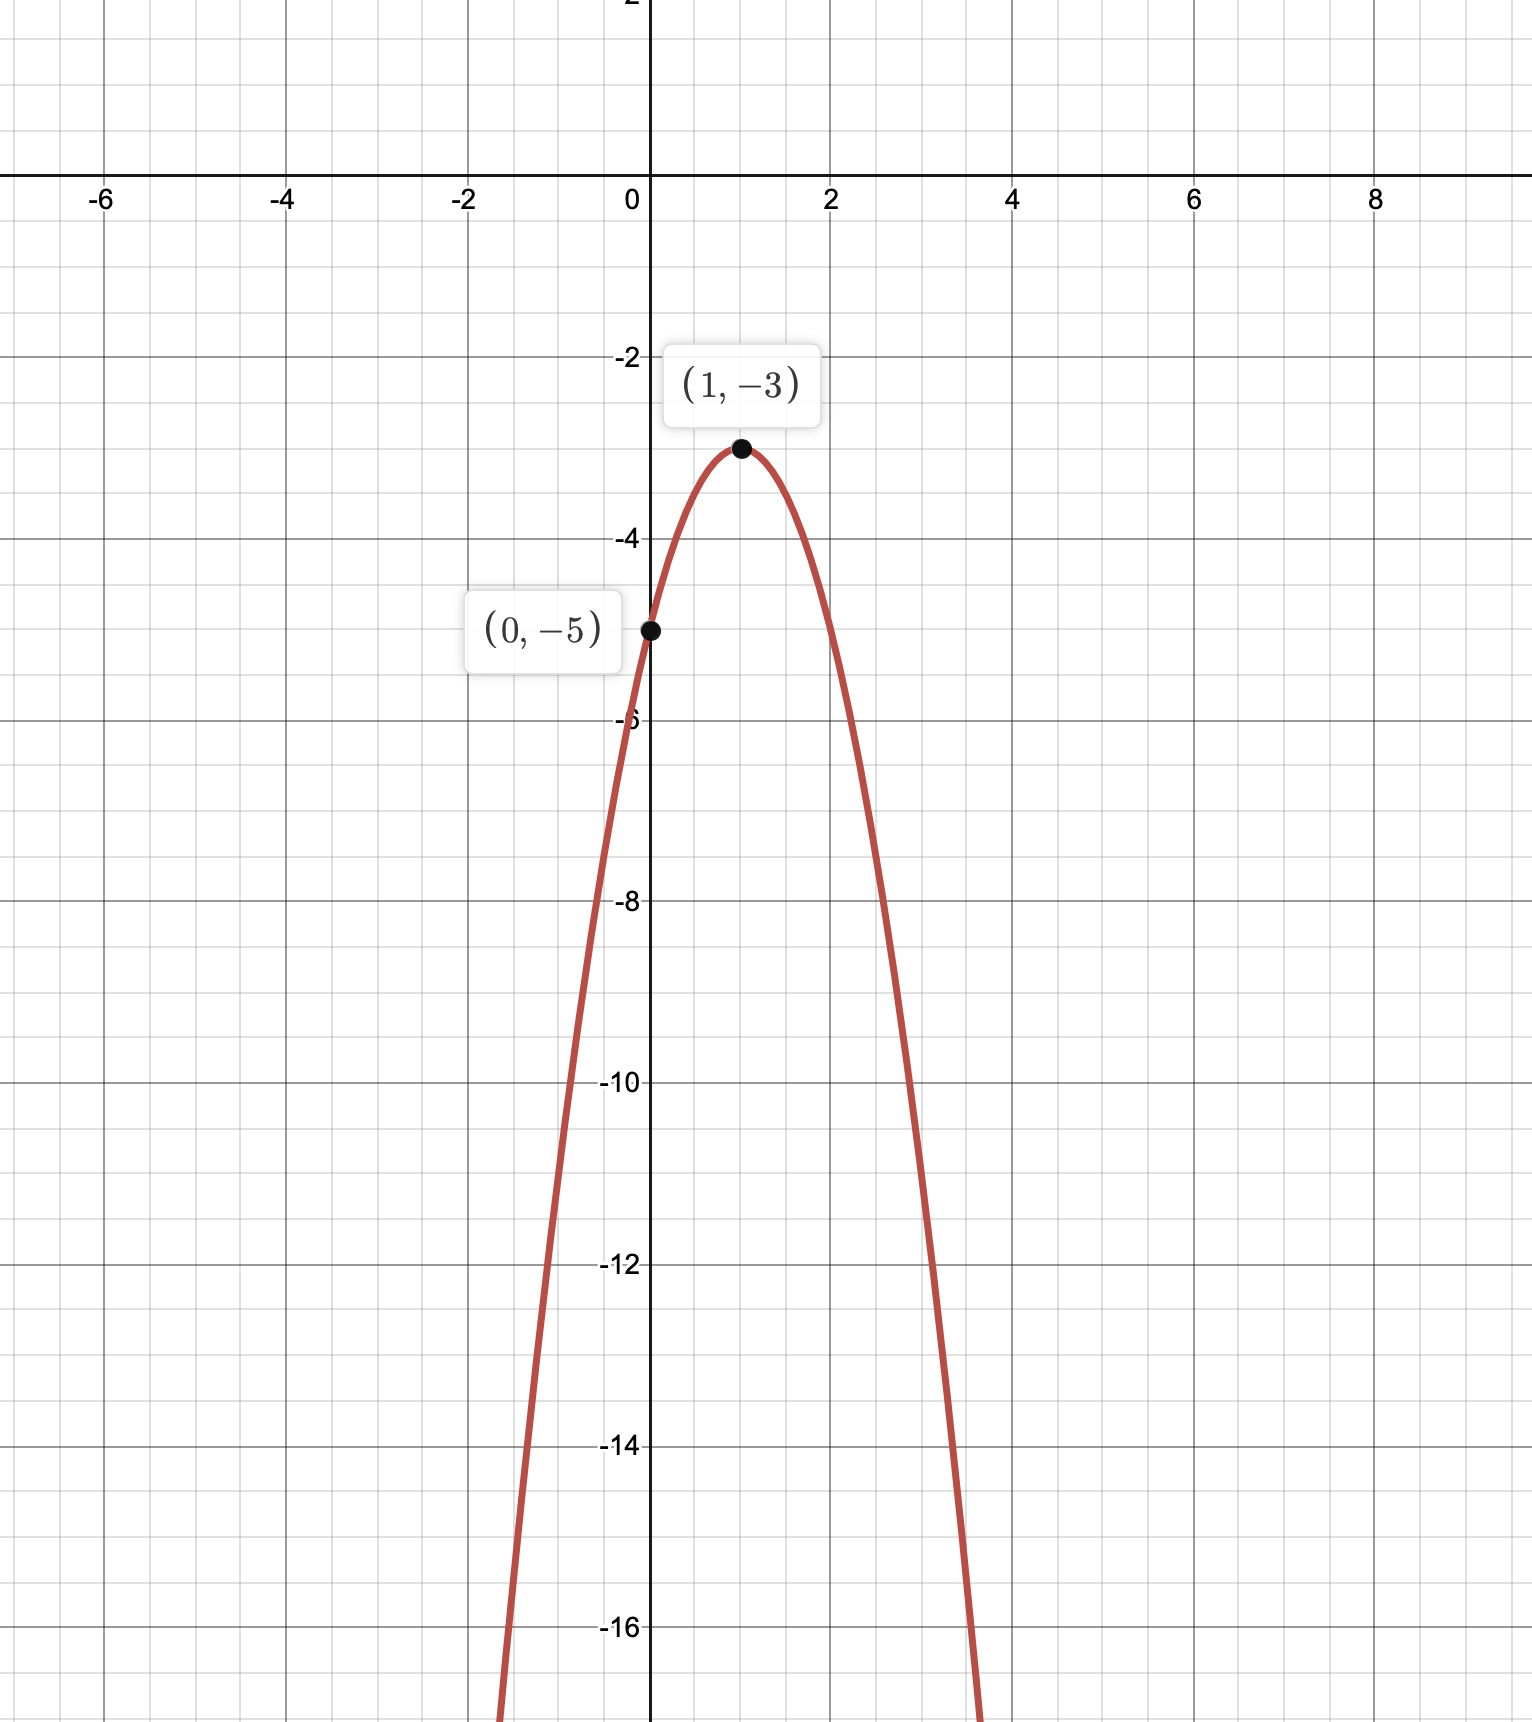
\includegraphics[width=6cm]{parabola1.png}
\end{figure}


\item Below is a graph of a transformed function $g(x)$ with two points labeled for you.  The base function is $f(x)=x^2$.  Write the equation of $g(x)$.  
\begin{figure}[!h]
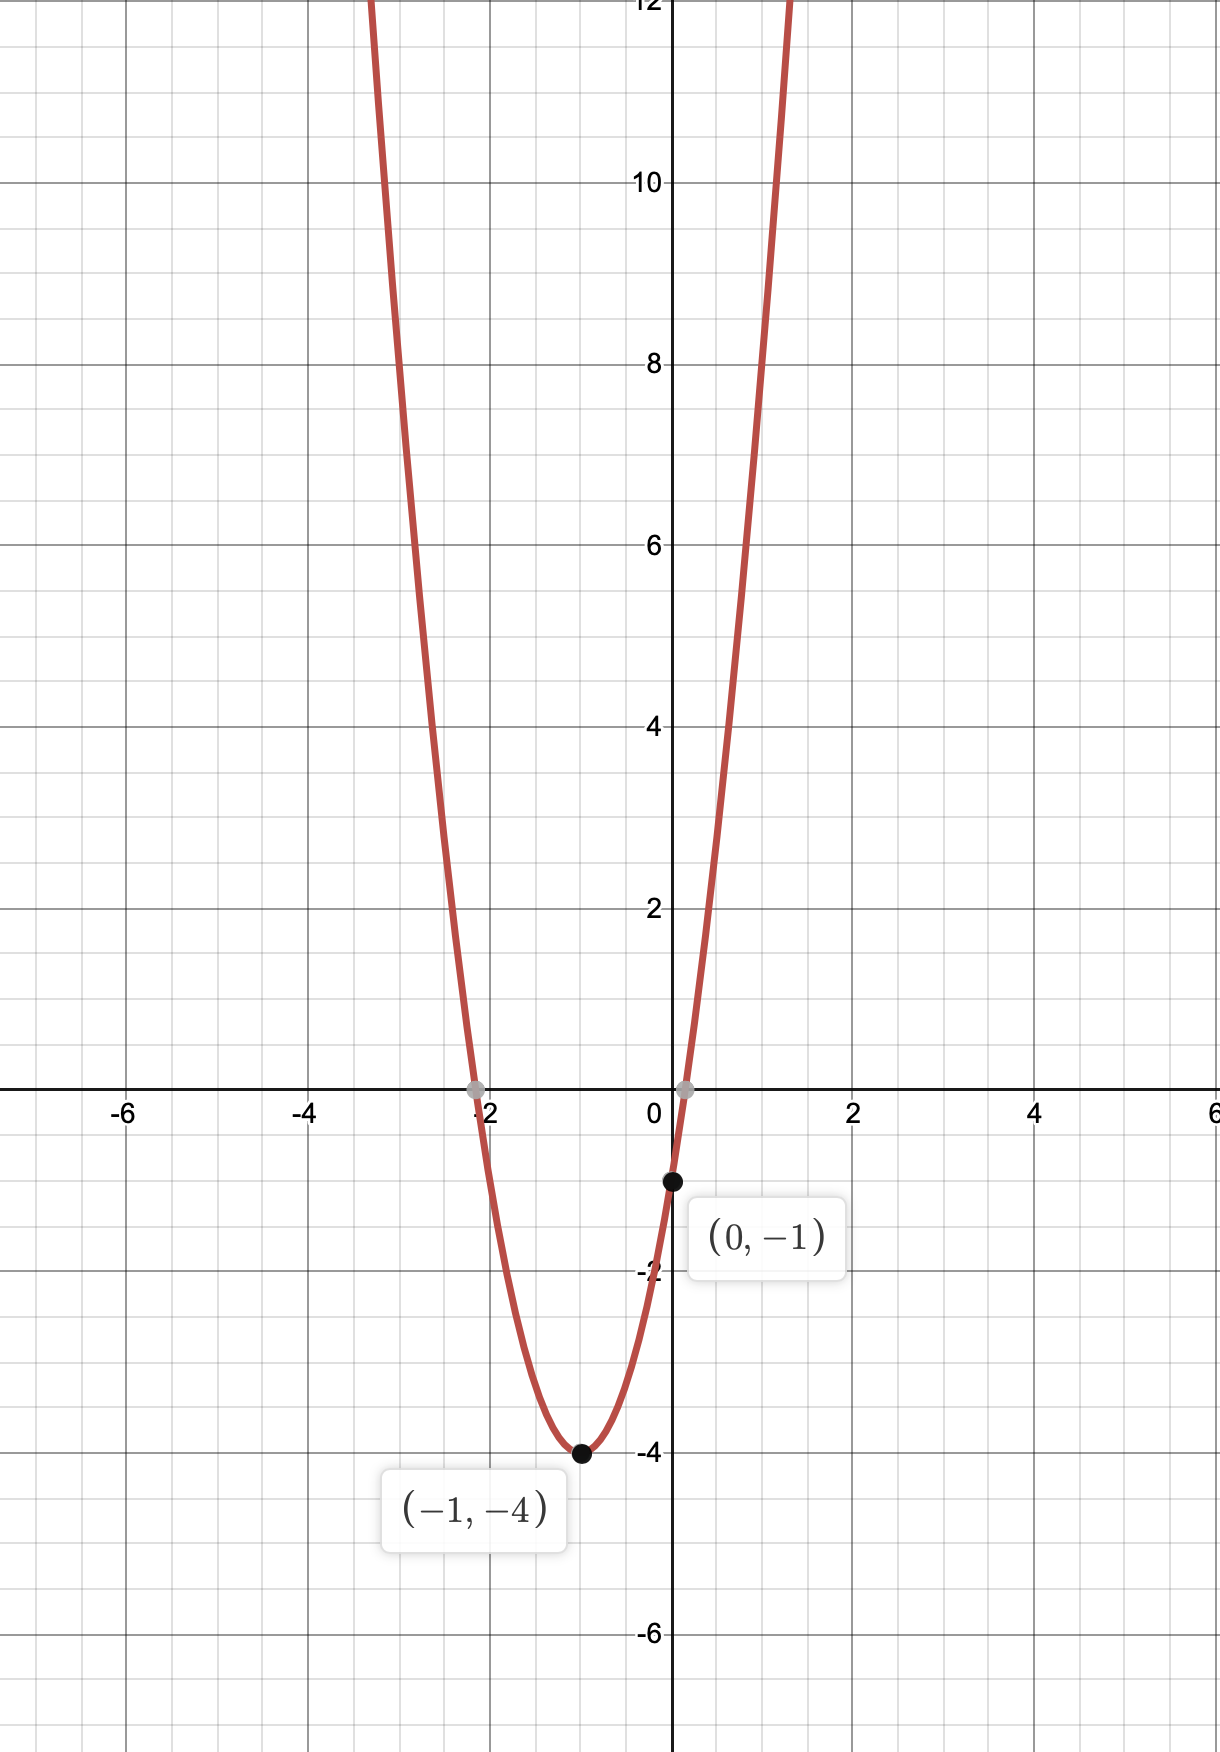
\includegraphics[width=6cm]{parabola2.png}
\end{figure}

\pagebreak

\item Below is a graph of a transformed function $g(x)$ with several points labeled for you.  The base function is $f(x)=\sqrt{x}$.  Write the equation of $g(x)$.  
\begin{figure}[!h]
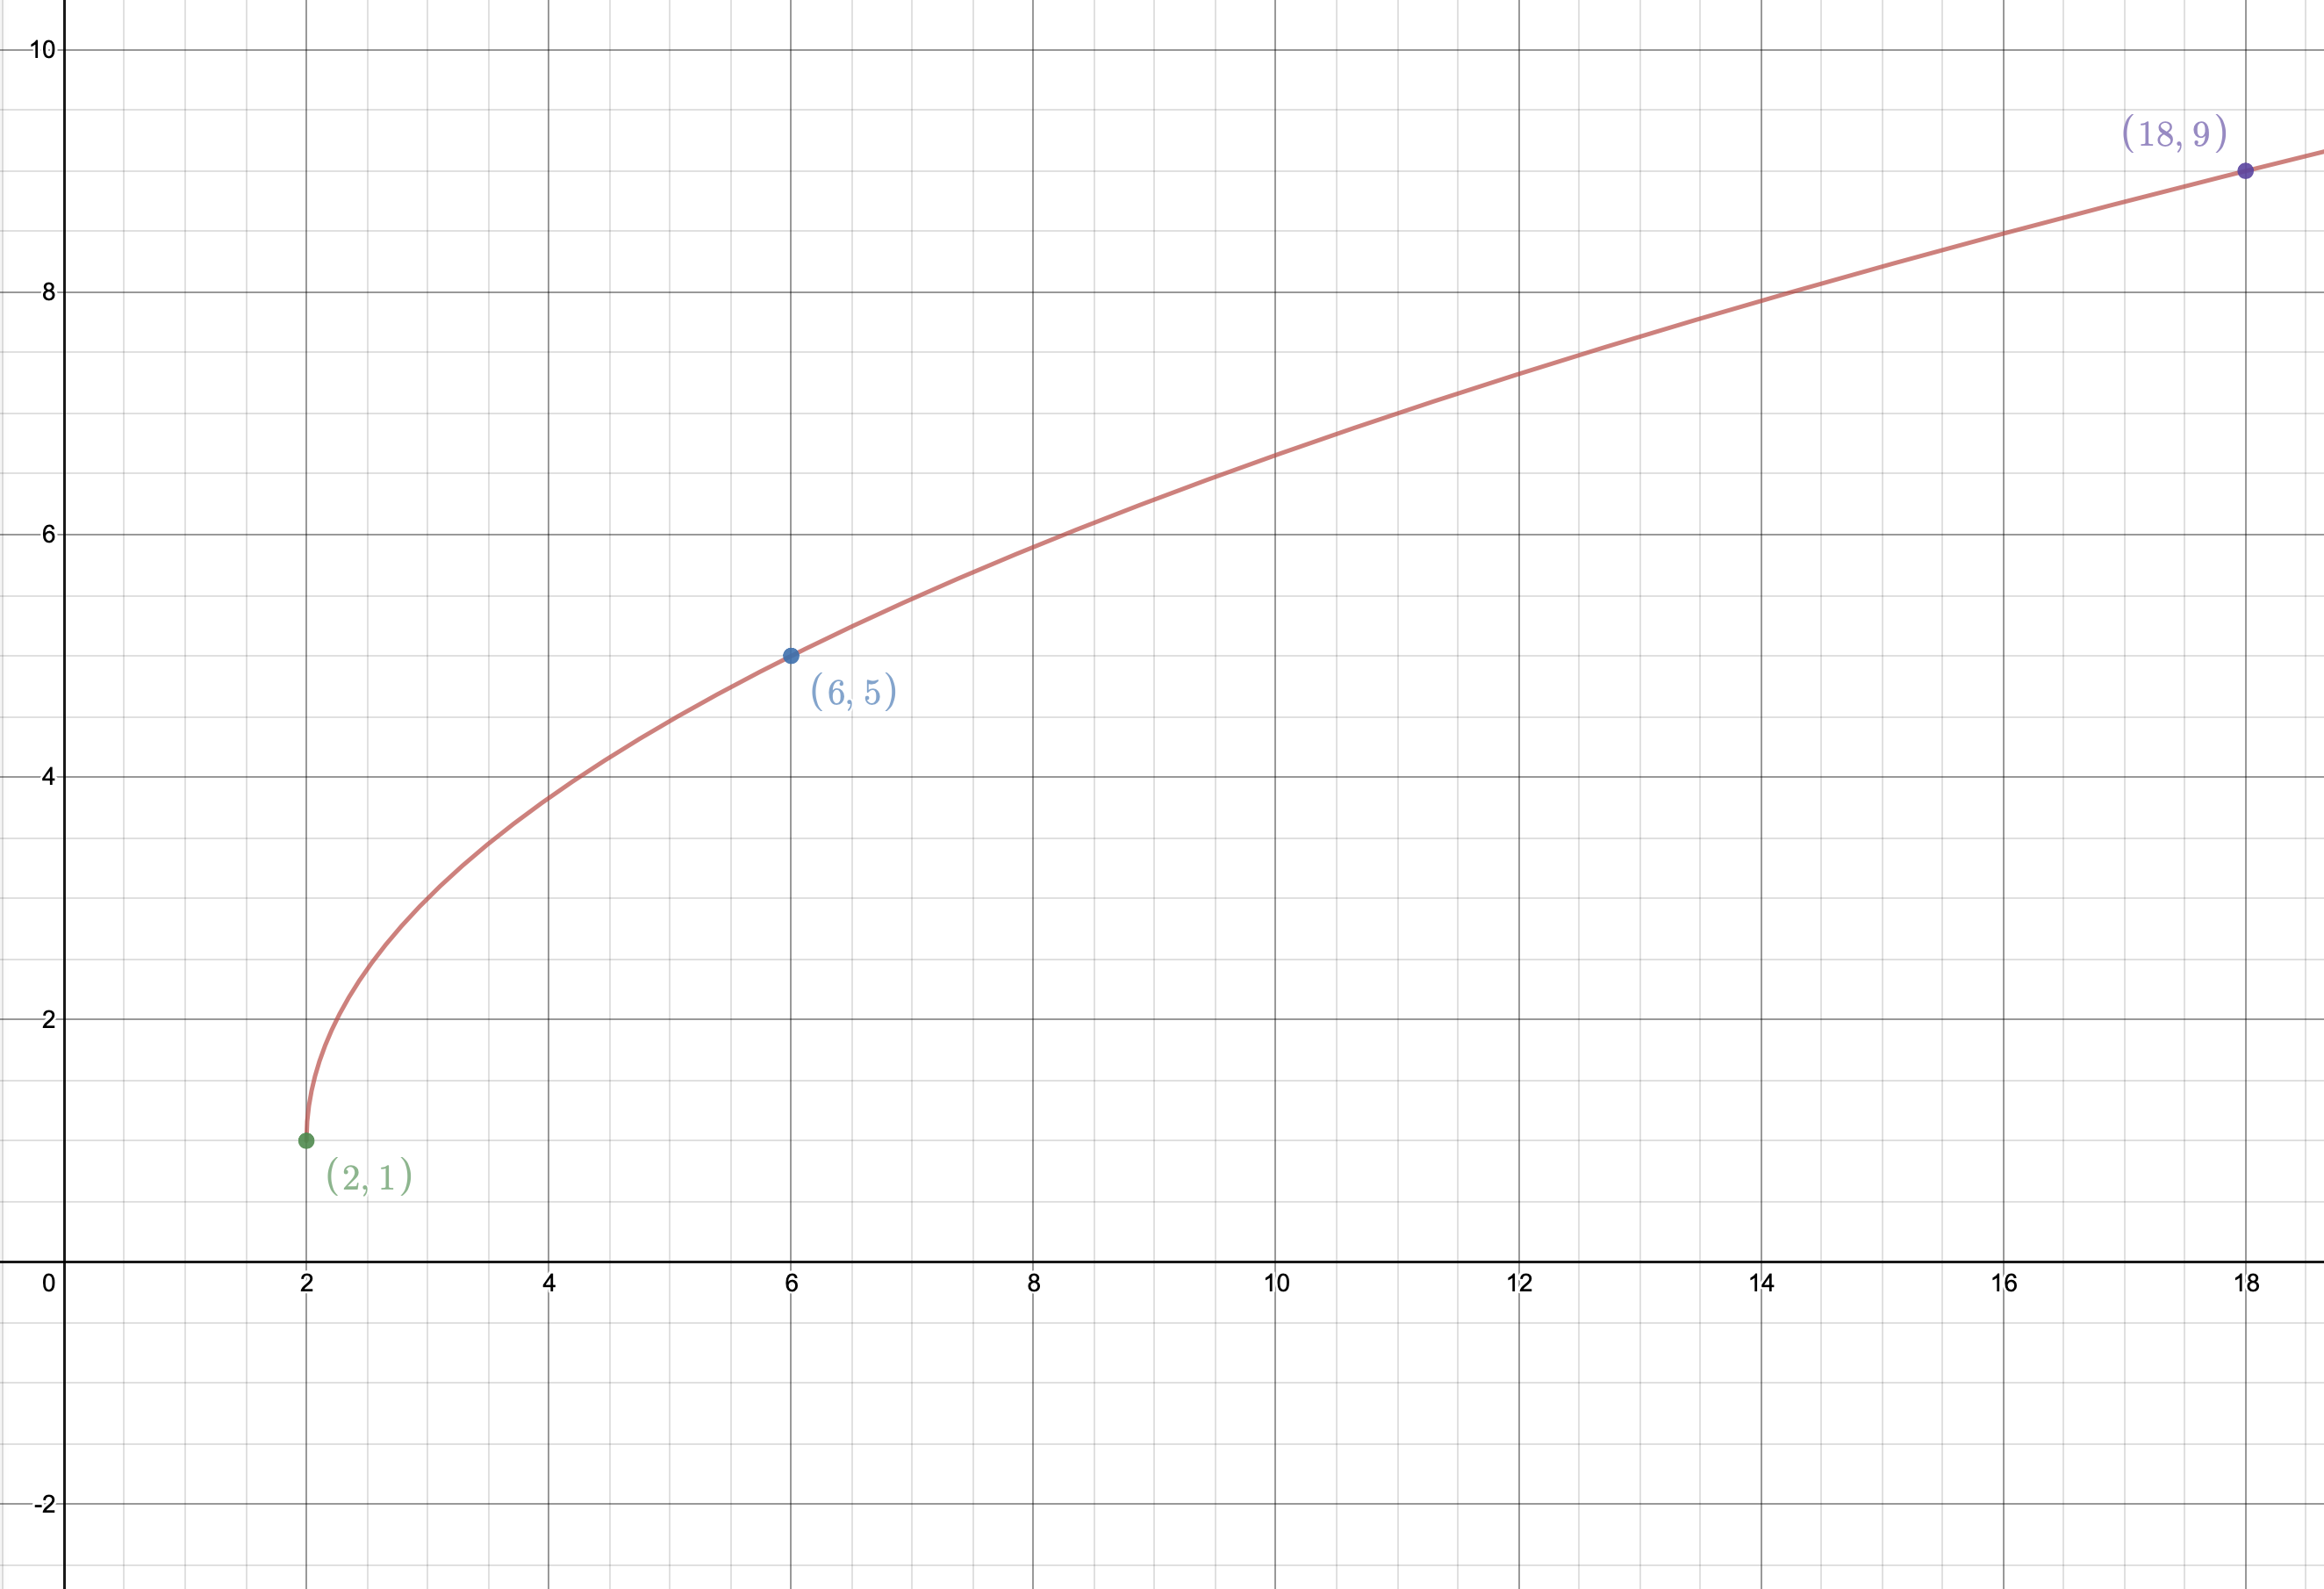
\includegraphics[width=6cm]{sqrt.png}
\end{figure}

 
\item REFLECTION AND CONSOLIDATION 
\begin{enumerate}
\item Summarize the main ideas/formulas you used for this problem set.  You can list formulas, bullet-out phrases, write a paragraph, draw sketches, or answer this question in any way that makes sense to you.
\item What three problems were the most challenging for you?  After deciding, look at your solutions carefully, and write a short explanation of what you found challenging and how you overcame this challenge in your problem solving.  For example, did you find a simpler problem about the same topic?  Did you guess and check?  Did you graph with technology?
\item Write three potential test questions on the topics covered in this problem set.
\end{enumerate}
      


\end{enumerate}


\end{document}